%----------------------------------------------------------------------------------------
%	PACKAGES AND OTHER DOCUMENT CONFIGURATIONS
%----------------------------------------------------------------------------------------

\documentclass{article} % Paper and 12pt font size
\usepackage[utf8]{inputenc}
\usepackage[T1]{fontenc}
% \usepackage{libertine}
\usepackage{lmodern} % Use font Latin Modern Sans Typewriter
% \renewcommand{\familydefault}{\ttdefault}
\usepackage[a4paper, margin=1in]{geometry} % Paper size and margin

\usepackage{enumitem} % Format the enumerated list
\usepackage{amsmath,amsfonts,mathtools} % Math packages
\usepackage{amsthm}
\interdisplaylinepenalty=2500
\usepackage{amssymb}
\usepackage[makeroom]{cancel}
\setlength\parindent{0pt} % Removes all indentation from paragraphs - comment this line for an assignment with lots of text

\usepackage{array}
\usepackage{tabu} % Table to text width
\renewcommand{\arraystretch}{1.} % The height of each row in the table is set to 1.5 relative to its default height.
\usepackage[table]{xcolor}

\usepackage{tikz} % Remember picture
\usepackage{graphicx} % Includes images
\graphicspath{ {./images/} } % Tells LATEX that the images are kept in a folder named images under the directory of the main document
\usepackage{wrapfig} % Wrap image i
\usepackage{eso-pic} % used for image background on titlepage


% Code listing style --------------
\usepackage{listings} % Code listing
\usepackage{color}
\definecolor{codegreen}{rgb}{0,0.6,0}
\definecolor{codegray}{rgb}{0.5,0.5,0.5}
\definecolor{codepurple}{rgb}{0.58,0,0.82}
\definecolor{backcolour}{rgb}{0.95,0.95,0.92}
\lstdefinestyle{mystyle}{
    backgroundcolor=\color{backcolour},
    commentstyle=\color{codegreen},
    basicstyle=\ttfamily\small,
    keywordstyle=\color{magenta},
    numberstyle=\tiny\color{codegray},
    stringstyle=\color{codepurple},
    breakatwhitespace=false,
    breaklines=true,
    captionpos=b,
    keepspaces=true,
    numbers=left,
    numbersep=5pt,
    showspaces=false,
    showstringspaces=false,
    showtabs=false,
    tabsize=2
}
\lstset{style=mystyle}
\usepackage{todonotes}  % Todo



%----------------------------------------------------------------------------------------
%	TITLE SECTION
%----------------------------------------------------------------------------------------
\title{\Huge \textbf{ASSIGNMENT 1} \vspace{.4in} \hrule}

\author{
	\Large ROB521: Mobile Robotics and Perception\\
	\Large Jojo (Yizhi) Zhou, 1003002396\\
}
\date{\normalsize\today}

\linespread{1.3}

\begin{document}
\fontfamily{lmtt} % modern typewriter font

%----------------------------------------------------------------------------------------
%	FRONT MATTER
%----------------------------------------------------------------------------------------
\begin{titlepage}
\tikz[remember picture,overlay]
\node[opacity=1] at (current page.center){
\includegraphics[width=\paperwidth,height=\paperheight]{../Background}};
\vspace*{3.5cm}
{\let\newpage\relax\maketitle}
\vspace*{\fill}

\end{titlepage}

% \newpage
\fontfamily{lmtt} % modern typewriter font

%----------------------------------------------------------------------------------------
%	Q1
%----------------------------------------------------------------------------------------
\section{Noise-free Wheel Odometry} % The * makes it an unnumbered section
\begin{figure}[hbt]
  \centering
    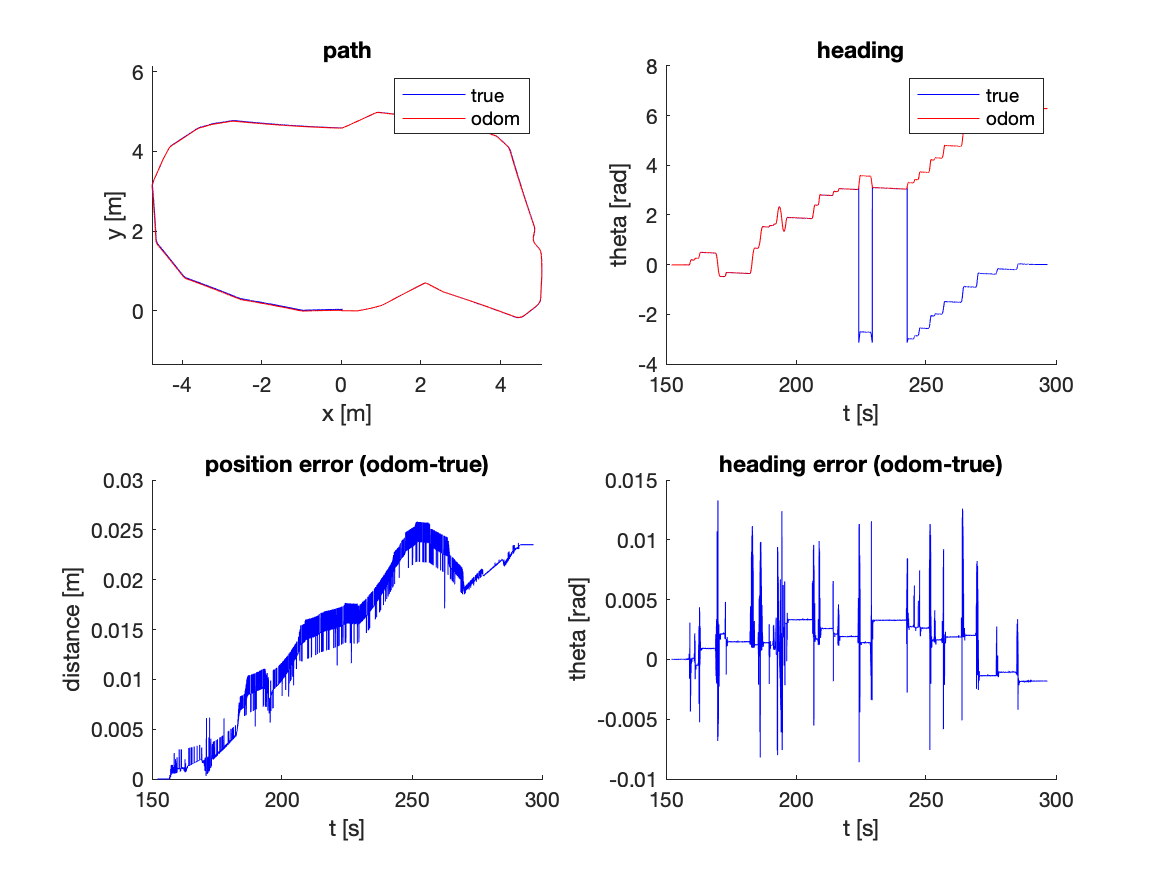
\includegraphics[width=1.0\textwidth]{ass1_q1.png}
  \caption{Output plot from to Question 1}
\end{figure}

The plot of the position is identical to the ground. As expected from noise free data, there is little to none uncertainty in the wheel encoder readings. There is very little offset from the true path taken, though the position error does still increase over time. Most of the error likely comes from the finite nature of the data as there is no noise or slippage in the encoder readings.
The most notable error is the heading of the robot which diverges from the ground truth at the middle and end of the trajectory. This is likely due to the way the robot measures the ground truth heading.
Since the odometry algorithm is incremental, it is impossible for the heading to suddenly jump by two pi. The measured, true heading on the other hand is effected by the specifications of the sensor or Gazebo software, allowing discrete jumps of two pi in the heading.
Compared to the solution image, the position pretty much identical to the solution image. The most notable difference is the heading; where as my solution differs from the ground truth by two pi, the sample solution follows the true heading perfectly. This indicates a difference in the sample solution algorithm implementation, through for the purposes of the calculated trajectory this is not important.

%----------------------------------------------------------------------------------------
%	Q2
%----------------------------------------------------------------------------------------
\section{Noisy Wheel Odometry} % The * makes it an unnumbered section
\begin{figure}[hbt]
  \centering
    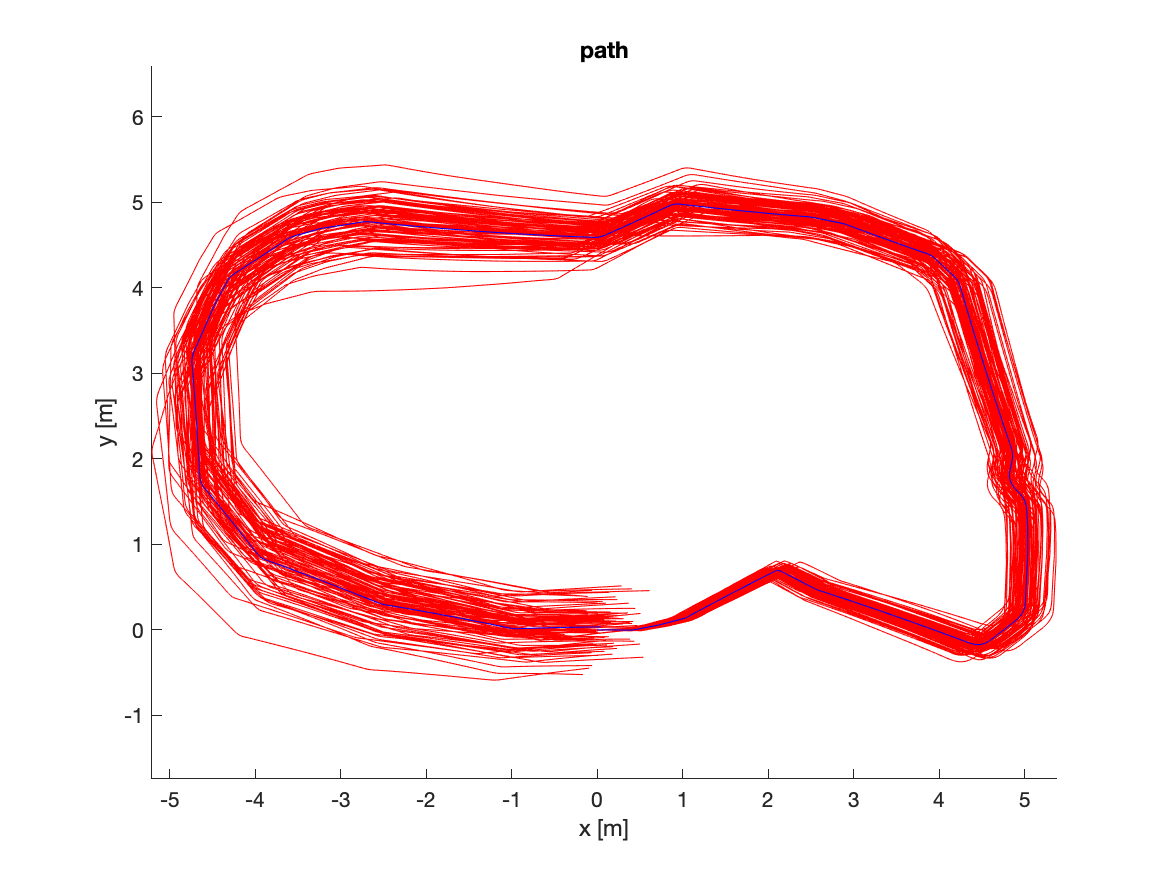
\includegraphics[width=0.9\textwidth]{ass1_q2.png}
  \caption{Output plot from to Question 2}
\end{figure}

As we can see from the numerous odometry runs, the divergence of the odometry pose from the true path grows over distance travel. While the mean of the 100 runs is centered around the ground truth, the final position error for some of the paths is close to 1 meter, indicating high uncertainty.
If we view the multiple runs as particles, we see the uncertainty grow without bound as the particles spread further apart and there is no way to tell which of the possible trajectories is the correct one.
The image looks identical the sample solution image so no comments will be made.

%----------------------------------------------------------------------------------------
%	Q3
%----------------------------------------------------------------------------------------
\section{Map from  Odometry} % The * makes it an unnumbered section
\begin{figure}[hbt]
  \centering
    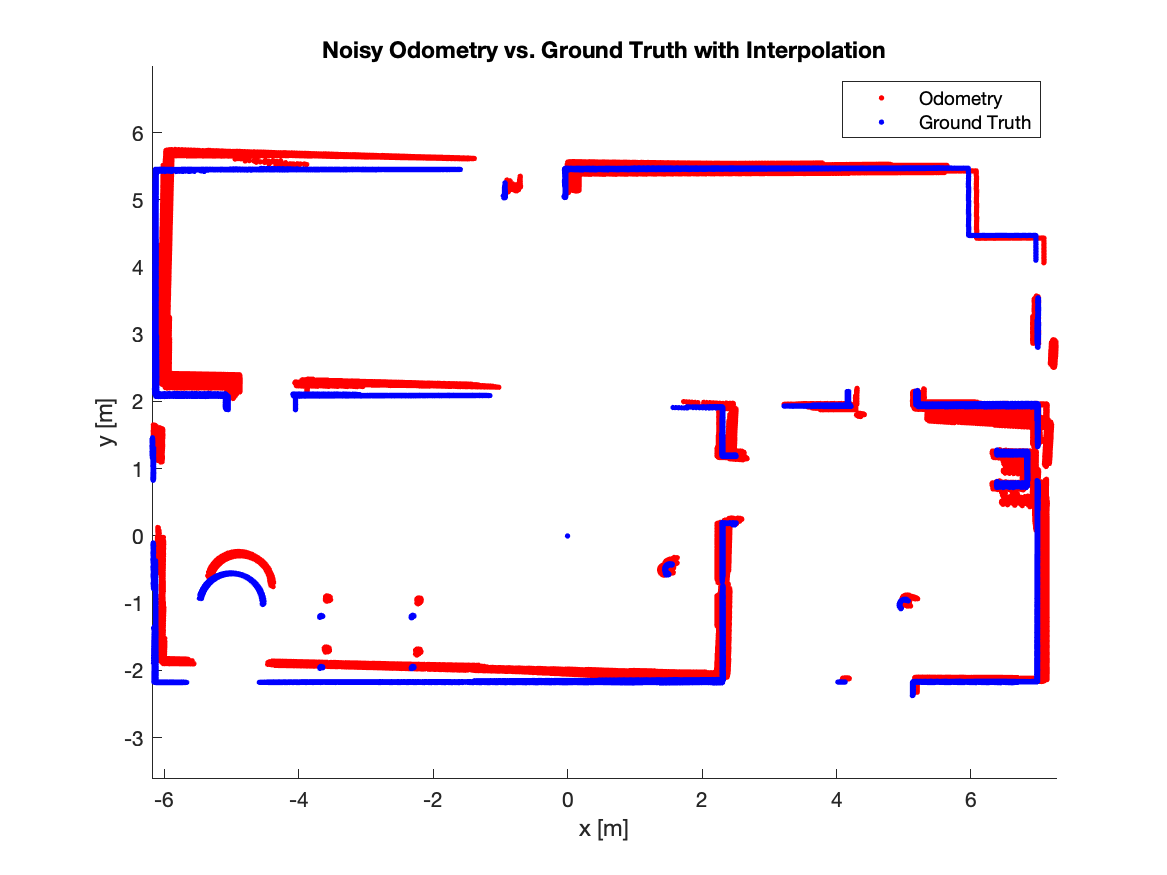
\includegraphics[width=0.9\textwidth]{ass1_q3.png}
  \caption{Output plot from to Question 3}
\end{figure}

For the noisy odometry data, the laser data gets more uncertain the longer the robot travels. This is expected as the odometry is a form of dead reckoning so the variance/uncertainty grows without bound. We can see growing errors in both the mean, as the odometry data is offset from the ground truth and sometime duplicated, and the variance, as the odometry landmarks are significantly thicker which indicates higher uncertainty.
While the two patches for angular velocity and laser position offset was applied, the resulting solution is still not as crisp as the sample solution. This does not appear to be simply a plotting error as the top-left corner is doubled in both plots, indicating some pose estimation errors in my algorithm.


%----------------------------------------------------------------------------------------
%	Appendix
%----------------------------------------------------------------------------------------
\clearpage
\section*{Appendix: Source Code}
\lstinputlisting[language=matlab]{ass1.m}


\end{document}
